% Implementation chapter continued
\section{Internals}\label{internals}
\subsection{RabbitMQ as a Central Message Bus}\index{RabbitMQ as a Central Message Bus}
\begin{figure}[h!]
  \centering
  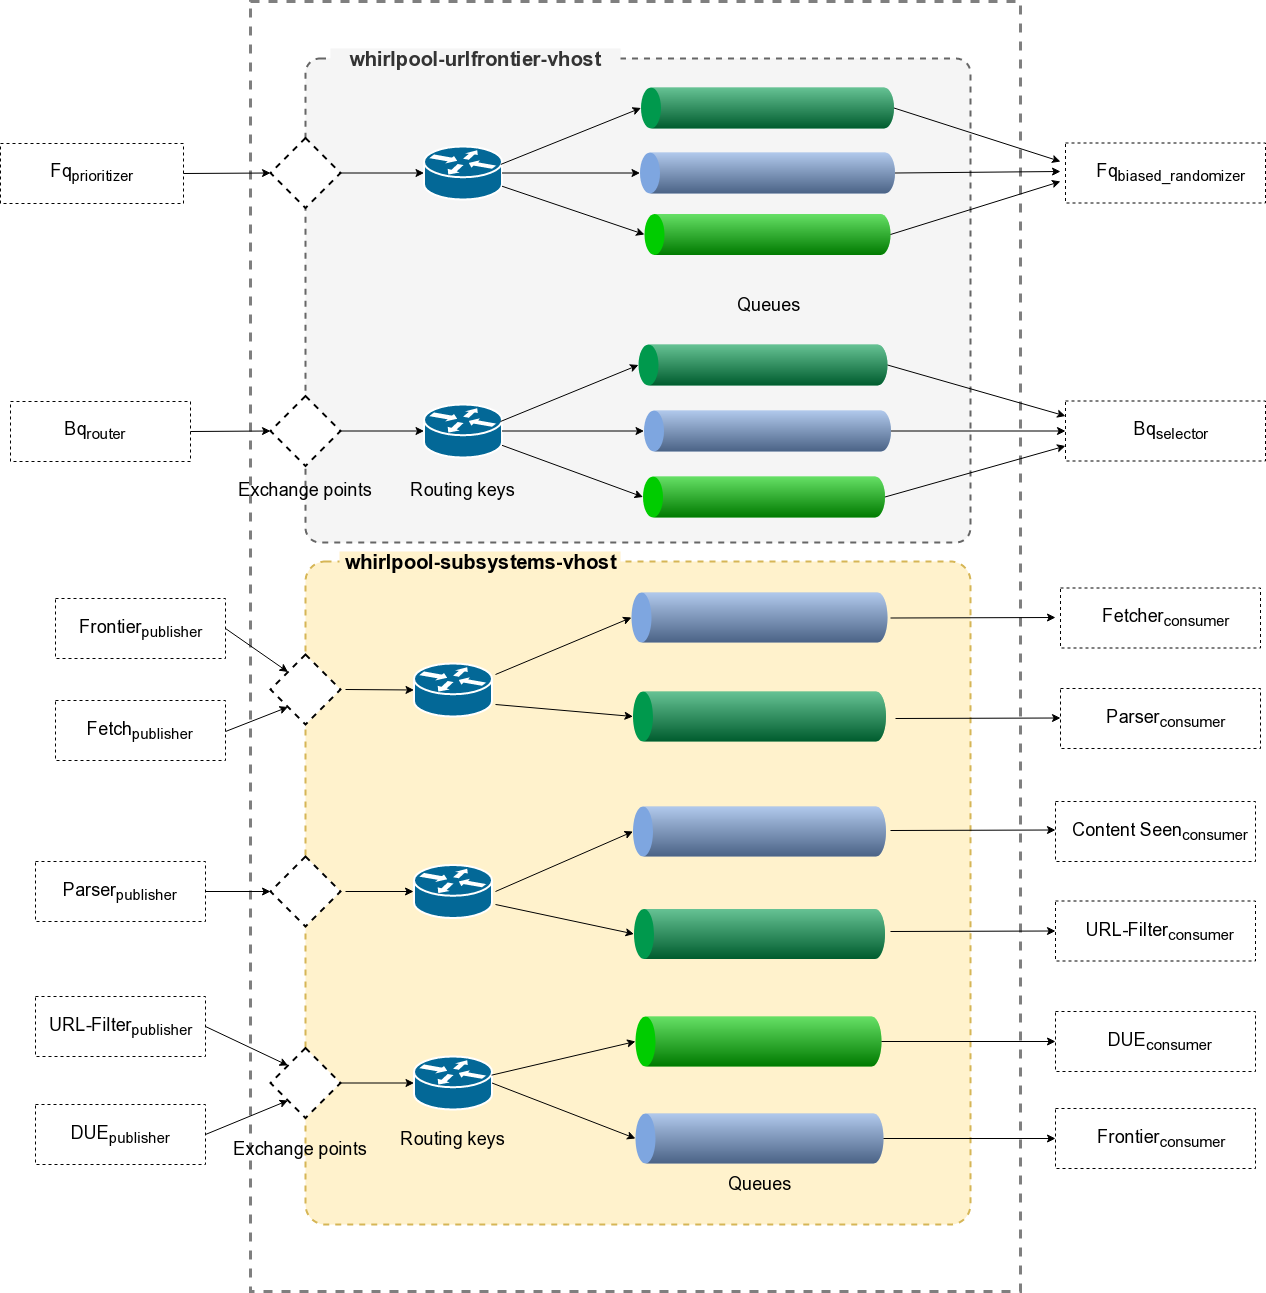
\includegraphics[width=20cm,height=15cm,keepaspectratio]{../media/crawler/rmq-broker.png}
  \caption{Message Distribution using RabbitMQ Direct Exchange}
  \label{fig:rmq}
\end{figure}

\noindent
The initial rabbitmq configuration is shown in the \url{https://github.com/rihbyne/whirlpool-rmq/blob/master/setup.j}. The subsystems only need to know the exchange points and submit message payload to it. The exchange points take care of routing payload to its recipient queue. The payload is static, and doesn't contain any business logic, this leaves the subsystems highly decoupled from each other.
\pagebreak

\subsection{Shared Services with Docker}\index{Shared Services with Docker}
\begin{figure}[h!]
  \centering
  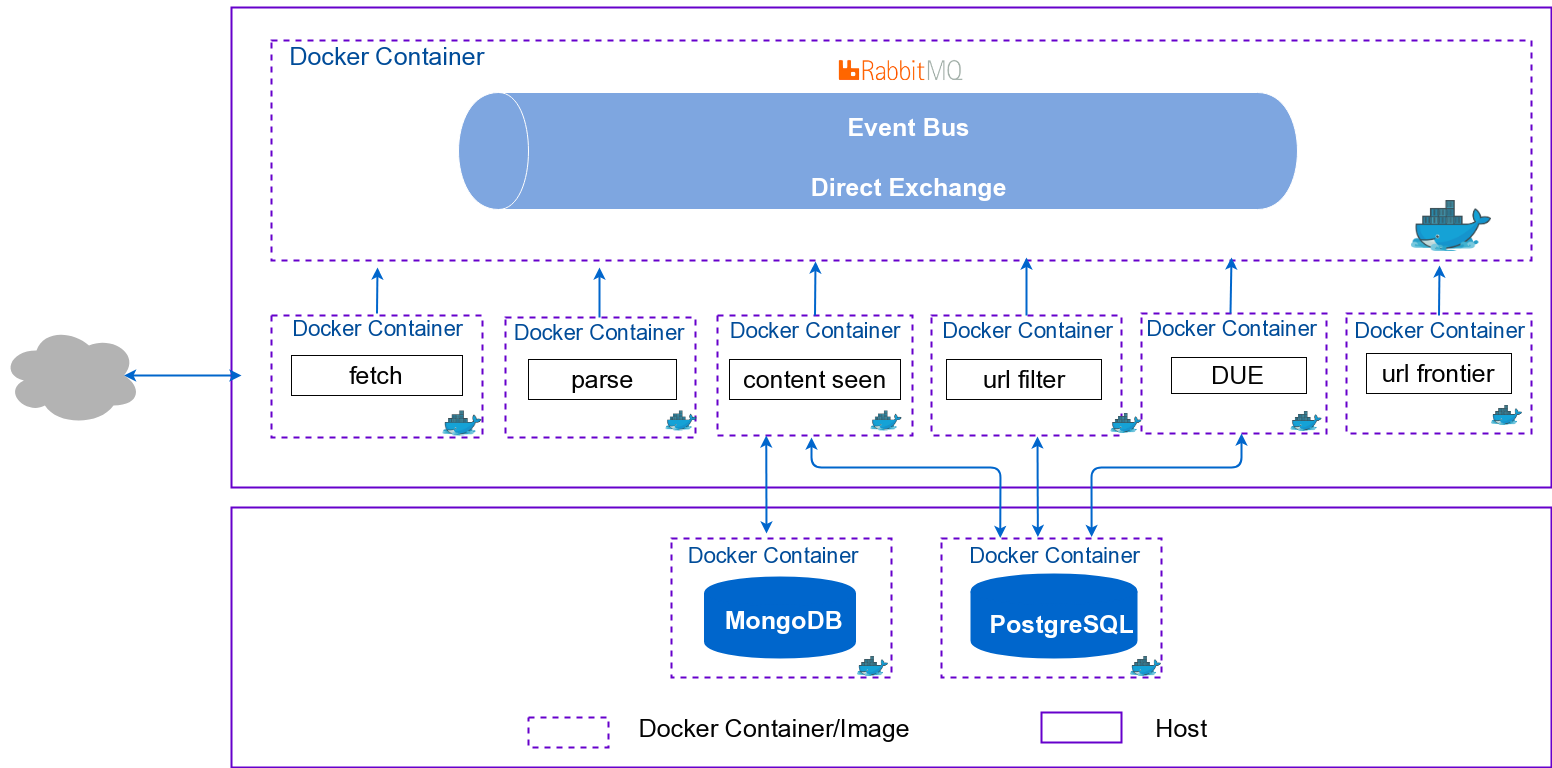
\includegraphics[width=18cm,height=10cm,keepaspectratio]{../media/crawler/multi-container-deploy.png}
  \caption{Single-node Whirlpool Subsystem Isolation using Docker}
  \label{fig:multicontainer}
\end{figure}

\pagebreak

\subsection{Developing code with Docker}\label{devdocker}
At the foundation of any dockerized program, \texttt{dockerfile} is a place to package source code. The biggest advantage of using containerization as discussed in section \ref{dockerintro}, is to get same program behavior under development and production environments, making deployment process easier. At first, a developer will use \texttt{dockerfile} for developmental use. This approach, however, is time-consuming, slows speedy development as docker engine takes a while to build \& re-run on every change. Whats even worse is that the size of development image gets bigger on each build as dependencies are added/removed, updates to the base images are installed. This actions aren't required when developing code. 
\\
\\
The best practice when developing code with docker is to use \texttt{docker-compose.yml} to define the environment at different layers. The version 2 of compose file allows to extend and reuse existing layers. Version 2 is more developer friendly while
version 3 is geared towards production use. As you can in below image under
\texttt{services} directive - install and quick-up project services extend base
project.

\inputminted[
fontfamily=tt,
baselinestretch=1.2,
fontsize=\footnotesize,
linenos,
breaklines,
numbersep=5pt,
tabsize=2,
firstline=1,
lastline=30,
frame=single]{yaml}{../../whirlpool/crawler/whirlpool-fetch/docker-compose.build.yml}

\pagebreak

\inputminted[
fontfamily=tt,
baselinestretch=1.2,
fontsize=\footnotesize,
linenos,
breaklines,
numbersep=5pt,
tabsize=2,
firstline=31,
lastline=34,
frame=single]{yaml}{../../whirlpool/crawler/whirlpool-fetch/docker-compose.build.yml}

\noindent
The environment defines external \texttt{network} sharing it with containers defined outside and inside the compose file. This is specific to development setup where 
one component is actively getting developed while others are in ready state. Similarly, the external \texttt{volume} persist javascript(in this example) dependencies outside the container, thus allowing sharing among other containers such as install and quick-up services.

\inputminted[
fontfamily=tt,
baselinestretch=1.2,
fontsize=\footnotesize,
linenos,
numbersep=5pt,
tabsize=2,
firstline=1,
lastline=14,
frame=single]{make}{../../whirlpool/crawler/whirlpool-fetch/Makefile}

\noindent
The use of \texttt{Makefile} makes docker commands easier to remember when typing on the command line. Note that the same commands can also be integrated into IDE of choice.

\begin{lstlisting}[language=bash]
  $ make install
\end{lstlisting}

\noindent
Trying the above command for the very first time will establish network, pull node image only once and install dependencies to the specified external volume. This is for the project defined in \texttt{docker-compose.build.yml}.

\begin{lstlisting}[language=bash]
  $ make quick-up
\end{lstlisting}

\noindent
Once the packages are installed, and after having made some changes to the code. The
program is launched using the above command. It runs inside the container with
installed packages shared by base servive. The flow is pretty fast as the install
and run operations are isolated and there is no time wasted in building and
packaging on every iteration of code change. This is very much ideal and
correct way to use docker while writing code.

\begin{lstlisting}[language=bash]
  $ make prod-build && make tag-prod && make push-prod
\end{lstlisting}
\noindent
This command clubs 3 commands - packages code for running on production machine, labels the image and pushes it to a central docker repository.

\pagebreak

\subsection{Policy of assigning priorities \& picking queues}
\begin{figure}[h!]
  \centering
  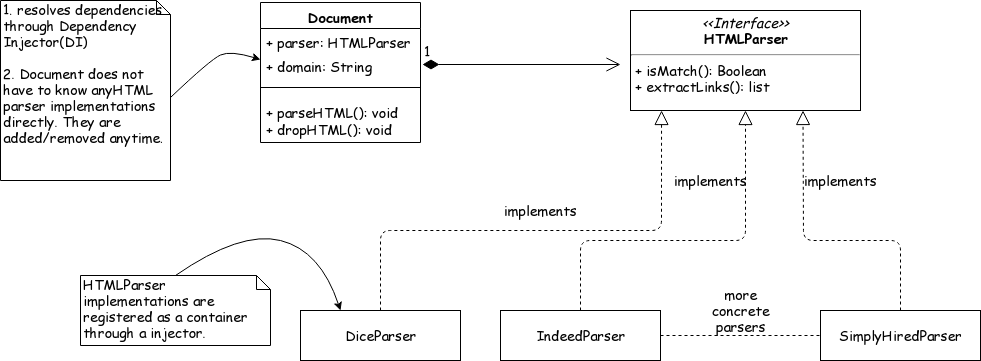
\includegraphics[width=15cm,height=12cm,keepaspectratio]{../media/crawler/docparsers.png}
  \caption{Whirlpool Parser subsystem using Dependency Injection}
  \label{fig:htmlparser}
\end{figure}

\pagebreak



